% !TEX TS-program = xelatex
% !BIB program = bibtex
% !TEX encoding = UTF-8 Unicode
% !Mode:: "TeX:UTF-8"
 \documentclass[bachelor, nocolorlinks, printoneside]{seuthesis} % 本科
% \documentclass[master]{seuthesis} % 硕士
% \documentclass[doctor]{seuthesis} % 博士
% \documentclass[engineering]{seuthesis} % 工程硕士
\usepackage{CJK,CJKnumb}
\usepackage{amsmath}
\usepackage{amsfonts} 
\usepackage{bm} 
\usepackage{algorithm}
\usepackage{algorithmicx}
\usepackage{algpseudocode}
\usepackage{subfigure}

\floatname{algorithm}{算法}
\renewcommand{\algorithmicrequire}{\textbf{输入:}}
\renewcommand{\algorithmicensure}{\textbf{输出:}}
 % 这里是导言区

\begin{document}
\categorynumber{000} % 分类采用《中国图书资料分类法》
\UDC{000}            %《国际十进分类法UDC》的类号
\secretlevel{公开}    %学位论文密级分为"公开"、"内部"、"秘密"和"机密"四种
\studentid{04016999}   %学号要完整,前面的零不能省略。

\title{东南大学本科毕业设计\LaTeX 模板}{}{SEU Thesis \LaTeX Template}{subtitle}
\author{林志 \& 侯宏卫}{Zhi Lin \& Hongwei Hou}
\advisor{神秘教授}{副教授}{No Name}{Associate Prof.}
\department{信息科学与工程学院}{Radio}
\major[12em]{信息工程}
\duration{2020年1月-2020年5月}

%\advisor{无名氏}{教授}{No Name}{Prof.}



\maketitle

\begin{abstract}{希腊字母,腓尼基字母,语言,深度学习}
注意!注意!注意!\LaTeX 读作latehe拉泰赫!

希腊字母源自腓尼基字母。腓尼基字母只有辅音,从右向左写。希腊语的元音发达,希腊人增添了元音字母。因为希腊人的书写工具是蜡板,有时前一行从右向左写完后顺势就从左向右写,变成所谓“耕地”式书写,后来逐渐演变成全部从左向右写。字母的方向也颠倒了。罗马人引进希腊字母,略微改变变为拉丁字母,在世界广为流行。希腊字母广泛应用到学术领域,如数学等。

希腊字母是希腊语所使用的字母,是世界上最早的有元音的字母,也广泛使用于数学、物理、生物、天文等学科。俄语等使用的西里尔字母也是由希腊字母演变而成。希腊字母进入了许多语言的词汇中,英语单字“alphabet”(字母表),源自拉丁语“alphabetum”,源自希腊语“αλφαβητον”,即为前两个希腊字母α(“Alpha”)及β(“Beta”)所合成,三角洲(“Delta”)这个词就来自希腊字母Δ,因为Δ是三角形。
\end{abstract}

\begin{englishabstract}{Greek Alphabet, Phoenician Alphabet, Language, Deep Learning}
The Greek alphabet has been used to write the Greek language since the late 9th century BC or early 8th century BC It was derived from the earlier Phoenician alphabet, and was the first alphabetic script to have distinct letters for vowels as well as consonants. It is the ancestor of the Latin and Cyrillic scripts.Apart from its use in writing the Greek language, in both its ancient and its modern forms, the Greek alphabet today also serves as a source of technical symbols and labels in many domains of mathematics, science and other fields.

In its classical and modern forms, the alphabet has 24 letters, ordered from alpha to omega. Like Latin and Cyrillic, Greek originally had only a single form of each letter; it developed the letter case distinction between upper-case and lower-case forms in parallel with Latin during the modern era.
\end{englishabstract}

\tableofcontents

% \begin{terminology}
% \begin{table}[h]
% \renewcommand\arraystretch{1.5}
% %\Large
% \begin{tabular}{>{\LARGE}m{0.2\textwidth} <{\centering}m{0.7\textwidth}}
% a & 如同汉字起源于象形,拉丁字母表中的每个字母一开始都是描摹某种动物或物体形状的图画\\

% b&和A一样,字母B也可以追溯到古代腓尼基。在腓尼基字母表中B叫beth,代表房屋,在希伯来语中B也叫beth,也含房屋之意。\\

% c& 字母C在腓尼基人的文字中叫gimel,代表骆驼。它在字母表中的排列顺序和希腊字母Γ(gamma)相同,实际上其字形是从后者演变而来的。C在罗马数字中表示100。\\

% d&D在古时是描摹拱门或门的形状而成的象形符号,在古代腓尼基语和希伯来语中叫做daleth,是“门”的意思,相当于希腊字母Δ(delta)。\\

% \end{tabular}
% %\caption{my table}
% \end{table}
% \end{terminology}


\begin{Main} % 开始正文

\chapter{前言}
%\emph{在泛函分析中,卷积、旋积或摺积(英语:Convolution)是通过两个函数f 和g 生成第三个函数的一种数学算子,表征函数f 与g经过翻转和平移的重叠部分的面积。}

\section{数学公式}
\subsection{简单的数学公式}
\textbf{卷积}(\textbf{convolution})在图像分析的线性方法中是一种重要的运算。卷积是一个积分,反映一个函数$f(t)$在另一个函数上$h(t)$移动时所重叠的量。函数$f$和$h$在有限域$[0,t]$上的$1D$卷积$f*h$由下式给出:
 $$(f*h)(t) \equiv \int_0^t {f(\tau )h(t - \tau )d\tau } $$

\subsection{带自动编号的公式}
这里可以限定在$[0,t]$区间,原因是我们假设负坐标部分的值是0。为了准确起见,我们还可以将卷积积分的上限扩展为$( - \infty ,\infty )$:
\begin{equation}(f*h)(t) \equiv \int_{ - \infty }^\infty  {f(\tau )h(t - \tau )d\tau }  = \int_{ - \infty }^\infty  {f(t - \tau )h(\tau )d\tau }
  \end{equation} 

\subsection{带等号对齐的公式}
卷积可以推广到更高维。令$2D$函数$f$和$h$的卷积$g$记为$f*h$,则有:
\begin{equation}
\begin{aligned}
(f*h)(x,y) &= \int_{ - \infty }^\infty  {\int_{ - \infty }^\infty  {f(a,b)h(x - a,y - b)} } dadb\\
 &= \int_{ - \infty }^\infty  {\int_{ - \infty }^\infty  {f(x - a,y - b)h(a,b)} } dadb\\
\end{aligned}
\end{equation}

\section{伪代码}
在写论文的时候我们通常要写伪代码,伪代码里面有时甚至还要包含数学公式(如根号一类的)。伪代码会自动找一个比较好的位置插入图片。

\begin{algorithm}
    \caption{用归并排序求逆序数}
    \begin{algorithmic}[1] %每行显示行号
        \Require $Array$数组,$n$数组大小
        \Ensure 逆序数
        \Function {MergerSort}{$Array, left, right$}
            \State $result \gets 0$
            \If {$left < right$}
                \State $middle \gets (left + right) / 2$
                \State $result \gets result +$ \Call{MergerSort}{$Array, left, middle$}
                \State $result \gets result +$ \Call{MergerSort}{$Array, middle, right$}
                \State $result \gets result +$ \Call{Merger}{$Array,left,middle,right$}
            \EndIf
            \State \Return{$result$}
        \EndFunction
        \State
        \Function{Merger}{$Array, left, middle, right$}
            \State $i\gets left$
            \State $j\gets middle$
            \State $k\gets 0$
            \State $result \gets 0$
            \While{$i<middle$ \textbf{and} $j<right$}
                \If{$Array[i]<Array[j]$}
                    \State $B[k++]\gets Array[i++]$
                \Else
                    \State $B[k++] \gets Array[j++]$
                    \State $result \gets result + (middle - i)$
                \EndIf
            \EndWhile
            \While{$i<middle$}
                \State $B[k++] \gets Array[i++]$
            \EndWhile
            \While{$j<right$}
                \State $B[k++] \gets Array[j++]$
            \EndWhile
            \For{$i = 0 \to k-1$}
                \State $Array[left + i] \gets B[i]$
            \EndFor
            \State \Return{$result$}
        \EndFunction
    \end{algorithmic}
\end{algorithm}

\section{插入图片}
在使用该命令的时候,图片会自动找一个他觉得比较好的位置插入图片,我们就不需要担心前面改了文字之后后面的格式乱掉。
\begin{figure}[htbp!]
\centering 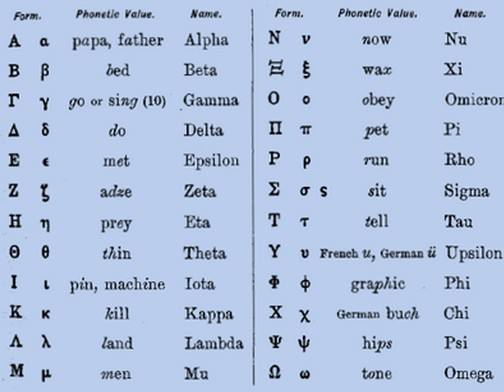
\includegraphics[width=0.9\textwidth]{img/test.jpg} \caption{图片的一个简单应用场景}
\end{figure}

\begin{figure}
\centering
\subfigure[the first subfigure]{
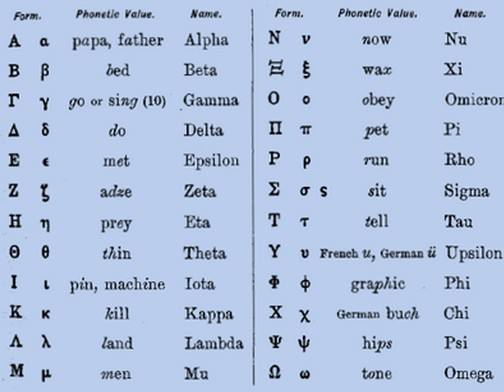
\includegraphics[width=0.4\textwidth]{img/test.jpg} 
}
\subfigure[the second subfigure]{
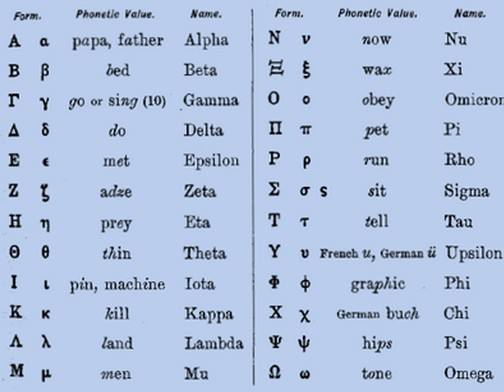
\includegraphics[width=0.4\textwidth]{img/test.jpg} 
}
\caption{子图应用场景}
\end{figure}

\section{引用论文}
使得论文符合要求\cite{Yao:2015ix}\cite{seucover}。

\chapter{研究内容}
\section{本章小结}

\end{Main} % 结束正文

% 参考文献
\bibliography{seuthesis}

%附录
\begin{Appendix}{}
    \chapter{{\LaTeX}实验}
    技术实验结果在这里写
    \chapter{MATLAB实验}
    技术实验结果在这里写
\end{Appendix}

\begin{Acknowledgement}{}
    这次的毕业论文设计总结是在我的指导老师xxx老师亲切关怀和悉心指导下完成的。从毕业设计选题到设计完成,x老师给予了我耐心指导与细心关怀,有了莫老师耐心指导与细心关怀我才不会在设计的过程中迷失方向,失去前进动力。x老师有严肃的科学态度,严谨的治学精神和精益求精的工作作风,这些都是我所需要学习的,感谢x老师给予了我这样一个学习机会,谢谢!

    感谢与我并肩作战的舍友与同学们,感谢关心我支持我的朋友们,感谢学校领导、老师们,感谢你们给予我的帮助与关怀;感谢肇庆学院,特别感谢计算机科学与软件学院四年来为我提供的良好学习环境,谢谢!
\end{Acknowledgement}

\newpage
\printindex % 索引

%\begin{thebibliography}{99}


%\bibliographystyle{ieee}
%\bibliography{seuthesis}


\end{document}
